\documentclass[../../main.tex]{subfiles}

\graphicspath{{../../image/}{../../figure/}}

\begin{document}

\section{概率法则}\label{section:ch02-概率法则}

在本节，我们将推导出两个控制概率行为的简单法则。虽然这两个法则看上去很简单，但我们将证明它们非常强大且具有广泛的适用性。首先我们通过一个简单的例子来引出概率法则。

\subsection{医学筛查示例}\label{subsection:ch02-医学筛查示例}

考虑对人群进行筛查以便尽早发现癌症患者的示例。假设人群中有 $1\%$ 的人患有癌症。理想情况下，我们的癌症检查对任何患有癌症的人都会给出阳性结果，而对任何未患癌症的人都会给出阴性结果。然而，癌症检查并不完美，所以我们假设当对未患癌症的人进行检查时，其中 $3\%$ 的人会被误判为阳性，这就是所谓的假阳性（false positive）。类似地，当检查那些确实患有癌症的人时，其中 $10\%$ 的人会被误判为阴性，这就是所谓的假阴性（false negative）。检查结果的准确性如\cref{figure:ch02-癌症检查}所示。

\begin{figure}[htbp]
  \centering
  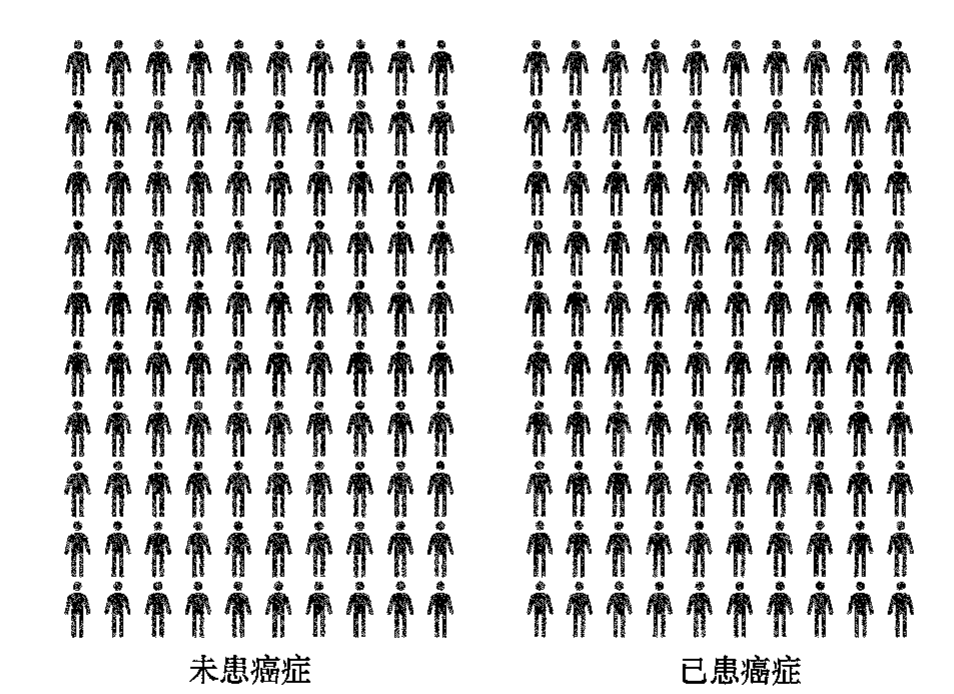
\includegraphics[width=0.52\textwidth]{ch02-fig2-3-cancer-test.png}
  \caption{癌症检查的准确性示意图。如左图所示，每 $100$ 名接受检查的未患癌症的人中，平均有 $3$ 人检查结果呈阳性。如右图所示，每 $100$ 名接受检查的患有癌症的人中，平均有 $90$ 人检查结果呈阳性。}
  \label{figure:ch02-癌症检查}
\end{figure}

有了这些信息，我们需要考虑以下问题：（1）如果我们对人群进行筛查，某人的检查结果呈阳性的概率是多少？（2）如果某人的检查结果呈阳性，那么他确实患有癌症的概率是多少？我们可以通过详细研究癌症筛查案例来回答这两个问题。但现在我们先不对这个例子做进一步讨论，而是首先推导出概率论的一般法则，即概率的加和法则和乘积法则。然后，我们将通过回答这两个问题来说明这两个法则具体是如何使用的。

\subsection{加和法则和乘积法则}\label{subsection:ch02-加和法则和乘积法则}

为了推导概率法则，\cref{figure:ch02-列联表}展示了一个更一般的例子，它涉及两个变量 $X$ 和 $Y$。在癌症检查的例子中，$X$ 表示癌症存在与否，$Y$ 表示检查结果变量。因为这两个变量的值可能以某种未知的方式因人而异，所以它们又称为随机变量（random variable 或 stochastic variable）。假设 $X$ 可以取任意值 $x_i$（其中 $i=1,\cdots,L$），并且 $Y$ 取值 $y_j$（其中 $j=1,\cdots,M$）。假设总共有 $N$ 次试验，我们同时对变量 $X$ 和 $Y$ 采样，并将 $X=x_i$ 且 $Y=y_j$ 的试验次数记为 $n_{ij}$。同样，记 $X$ 取值为 $x_i$（不考虑 $Y$ 的取值）的试验次数为 $c_i$，记 $Y$ 取值为 $y_j$ 的试验次数为 $r_j$。

\begin{definition}[随机变量]\label{definition:ch02-随机变量}
设一次试验的可能结果构成集合 $\Omega$（称为样本空间）。若对每个可能结果都指定了一个取值，则称这个取值为\textbf{随机变量}（random variable），也称随机变量（stochastic variable）。若随机变量 $X$ 只能取有限或可数多个值 $x_1,x_2,\cdots$，则称它为\textbf{离散的}；若它可以在某个区间上取任意实数值，则称它为\textbf{连续的}。把 $X$ 取值为 $x_i$ 这一事件记为 $X=x_i$。
\end{definition}

% SUPPLEMENT: parent=definition:ch02-随机变量; kind=motivation; location=紧随其后的 remark（重构新增）
\begin{remark}（重构新增）
随机变量不是“随机的数”，而是“从结果到数的映射”：正因如此，我们才能用 $X=x_i$ 这样的等式来叙述事件，并谈论它的频率。\cref{definition:ch02-随机变量}中“离散”与“连续”的划分决定了后文的叙述方式：离散情形用求和与计数（本节），连续情形用积分与概率密度（\cref{section:ch02-概率密度}）。

这里的关键条件是每一个结果都必须被指派一个确定的值——否则 $n_{ij}$ 无法定义，后面的频率解释也就无从建立。癌症检查的例子中，$C$ 与 $T$ 都是二值离散随机变量，这一点使得本节的所有论证都归结为对整数 $n_{ij}$ 的计数。
\end{remark}

\begin{figure}[htbp]
  \centering
  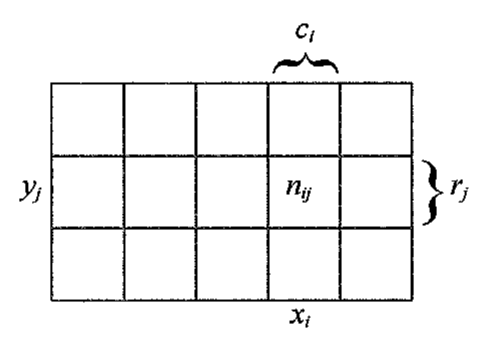
\includegraphics[width=0.38\textwidth]{ch02-fig2-4-contingency.png}
  \caption{通过考虑随机变量 $X$（$X$ 取值为 $\{x_i\}$，其中 $i=1,\cdots,L$）和 $Y$（$Y$ 取值为 $\{y_j\}$，其中 $j=1,\cdots,M$）来推导概率的加和法则和乘积法则。其中，$L=5$，$M=3$。如果考虑总共 $N$ 个实例中的这些变量，则用 $n_{ij}$ 表示 $X=x_i$ 和 $Y=y_j$ 的实例数，这是阵列中对应单元格的实例数。用 $c_i$ 表示第 $i$ 列对应于 $X=x_i$ 的实例数，用 $r_j$ 表示第 $j$ 行对应于 $Y=y_j$ 的实例数。}
  \label{figure:ch02-列联表}
\end{figure}

$X$ 取值为 $x_i$ 且 $Y$ 取值为 $y_j$ 的概率记为 $p(X=x_i,Y=y_j)$，称作 $X=x_i$ 和 $Y=y_j$ 的联合（joint）概率。它由落在单元格 $(i,j)$ 中的点数占总点数的比例给出，因此有

\begin{align}
  p(X=x_i,Y=y_j) = \frac{n_{ij}}{N}
  \label{align:ch02-联合概率定义}
\end{align}

\begin{definition}[联合概率与边缘概率]\label{definition:ch02-联合概率}
设 $X$ 取值于 $\{x_1,\cdots,x_L\}$，$Y$ 取值于 $\{y_1,\cdots,y_M\}$。称 $X=x_i$ 与 $Y=y_j$ 同时成立的概率 $p(X=x_i,Y=y_j)$ 为 $X$ 与 $Y$ 的\textbf{联合概率}（joint probability）。称只关心 $X$ 取值、不考虑 $Y$ 取值时 $X=x_i$ 的概率 $p(X=x_i)$ 为 $X$ 的\textbf{边缘概率}（marginal probability）。把求边缘概率的过程（即对另一个变量的所有取值求和）称为\textbf{边缘化}（marginalization）。
\end{definition}

% SUPPLEMENT: parent=definition:ch02-联合概率; kind=motivation; location=紧随其后的 remark（重构新增）
\begin{remark}（重构新增）
引入这两个概念是为了把“同时发生”与“单独发生”区分开。联合概率 $p(X=x_i,Y=y_j)$ 描述的是\cref{figure:ch02-列联表}中单个单元格的占比 $n_{ij}/N$；边缘概率 $p(X=x_i)$ 描述的是整列的占比 $c_i/N$。正因为单元格的数目比列多得多，$p(X,Y)$ 的信息量比 $p(X)$ 大：由 $p(X,Y)$ 可以算出 $p(X)$，反之则不能。

条件“$Y$ 的所有可能取值都被求和掉”体现了边缘化的含义：边缘化是有损操作，它会丢掉 $X$ 与 $Y$ 之间的依赖关系。后文\cref{section:ch02-概率密度}中的连续情形把求和换成积分，定义本身不变。
\end{remark}

这里隐式地考虑了极限 $N\to\infty$。类似地，在不考虑 $Y$ 取值的情况下，$X$ 取值为 $x_i$ 的概率记为 $p(X=x_i)$，它由落在第 $i$ 列中的点数占总点数的比例给出，因此有

\begin{align}
  p(X=x_i) = \frac{c_i}{N}
  \label{align:ch02-边缘概率定义}
\end{align}

由于 $\sum_i c_i = N$，可以看出

\begin{align}
  \sum_{i=1}^{L} p(X=x_i) = 1
  \label{align:ch02-边缘概率归一化}
\end{align}

\begin{proposition}[边缘概率的归一化]\label{proposition:ch02-边缘概率归一化}
设离散随机变量 $X$ 取值于 $\{x_1,\cdots,x_L\}$，其边缘概率由\eqref{align:ch02-边缘概率定义}给出，则\eqref{align:ch02-边缘概率归一化}成立，即 $\sum_{i=1}^{L}p(X=x_i)=1$。
\end{proposition}

\begin{proof}
由\cref{figure:ch02-列联表}，$c_i$ 是第 $i$ 列中全部单元格的实例数之和，而各列互不重叠地覆盖了全部 $N$ 个实例，故 $\sum_{i=1}^{L}c_i=N$。代入\eqref{align:ch02-边缘概率定义}得
\begin{align*}
  \sum_{i=1}^{L} p(X=x_i) = \sum_{i=1}^{L}\frac{c_i}{N} = \frac{1}{N}\sum_{i=1}^{L}c_i = \frac{N}{N} = 1 .
\end{align*}
\end{proof}

% SUPPLEMENT: parent=proposition:ch02-边缘概率归一化; kind=motivation; location=紧随其后的 remark（重构新增）
\begin{remark}（重构新增）
归一化不是一条附加的技术假设，而是“全部实例被各列无重复地划分”这一计数事实的直接翻译：$\sum_i c_i=N$。它保证 $p(X)$ 是一个概率分布而不是任意的非负函数，因而后文用 $p(X)$ 作权重求期望、用 $1/p(x)$ 度量信息量时才有意义。

条件“各列互不重叠且覆盖全体”不可省：若同一个实例被计入两列（例如允许一个人同时属于两个年龄组），则 $\sum_i c_i>N$，归一化失败。这也是\cref{definition:ch02-随机变量}要求对每个结果指派唯一取值的原因。
\end{remark}

因此，概率之和为 $1$。因为在\cref{figure:ch02-列联表}中，第 $i$ 列的实例数就是该列每个单元格中实例数的总和，所以有 $c_i=\sum_j n_{ij}$。根据\eqref{align:ch02-联合概率定义}和\eqref{align:ch02-边缘概率定义}，有

\begin{align}
  p(X=x_i) = \sum_{j=1}^{M} p(X=x_i,Y=y_j)
  \label{align:ch02-加和法则离散}
\end{align}

这就是概率的加和法则。请注意，$p(X=x_i)$ 有时称为边缘（marginal）概率，它是通过边缘化或求和其他变量（在这里是 $Y$）得到的。

\begin{proposition}[加和法则（离散形式）]\label{proposition:ch02-加和法则离散}
设 $X$ 与 $Y$ 为离散随机变量，$X$ 取值于 $\{x_1,\cdots,x_L\}$，$Y$ 取值于 $\{y_1,\cdots,y_M\}$，则对每个 $i$，\eqref{align:ch02-加和法则离散}成立，即联合概率对 $Y$ 的全部取值求和给出 $X$ 的边缘概率。
\end{proposition}

\begin{proof}
由 $c_i=\sum_{j=1}^{M}n_{ij}$（\cref{figure:ch02-列联表}中第 $i$ 列的实例数等于该列各单元格实例数之和），并代入\eqref{align:ch02-联合概率定义}与\eqref{align:ch02-边缘概率定义}，
\begin{align*}
  \sum_{j=1}^{M} p(X=x_i,Y=y_j) = \sum_{j=1}^{M}\frac{n_{ij}}{N} = \frac{1}{N}\sum_{j=1}^{M}n_{ij} = \frac{c_i}{N} = p(X=x_i) .
\end{align*}
\end{proof}

% SUPPLEMENT: parent=proposition:ch02-加和法则离散; kind=motivation; location=紧随其后的 remark（重构新增）
\begin{remark}（重构新增）
加和法则的作用是把“高维的联合分布”压成“低维的边缘分布”，它是后文所有模型中对隐变量求和（例如\cref{section:ch02-Bayes概率}中计算分母）的依据。证明之所以只有一行，是因为离散情形的求和恰好就是计数；这一步在连续情形要换成积分，并在 $N\to\infty$ 的极限下由频率过渡为密度，见\cref{section:ch02-概率密度}。

条件“对 $Y$ 的全部取值求和”不可省：只对部分 $y_j$ 求和得到的是 $p(X=x_i,Y\in A)$，一般不等于 $p(X=x_i)$。此外，求和能够进行的前提是 $Y$ 的取值至多可数；否则必须换成积分。
\end{remark}

如果我们只考虑 $X=x_i$ 的实例，那么 $Y=y_j$ 的实例的占比可以记为 $p(Y=y_j\mid X=x_i)$，称作给定 $X=x_i$ 下 $Y=y_j$ 的条件（conditional）概率。它可以通过在第 $i$ 列中寻找落在单元格 $(i,j)$ 中的那些点的占比得到，因此，它可以由下式给出：

\begin{align}
  p(Y=y_j\mid X=x_i) = \frac{n_{ij}}{c_i}
  \label{align:ch02-条件概率定义}
\end{align}

\begin{definition}[条件概率]\label{definition:ch02-条件概率}
设 $p(X=x_i)>0$。称在已知 $X=x_i$ 成立的条件下 $Y=y_j$ 成立的概率为\textbf{条件概率}（conditional probability），记作 $p(Y=y_j\mid X=x_i)$，它由\eqref{align:ch02-条件概率定义}定义，即把考察范围限制在第 $i$ 列之内、再取单元格 $(i,j)$ 在该列中所占的比例。
\end{definition}

% SUPPLEMENT: parent=definition:ch02-条件概率; kind=motivation; location=紧随其后的 remark（重构新增）
\begin{remark}（重构新增）
条件概率回答的是“已知 $X$ 取某个值之后，$Y$ 的分布如何”，因此它把原来的样本空间 $N$ 个点替换成了第 $i$ 列的 $c_i$ 个点。这个“换分母”的动作是条件概率与联合概率的唯一差别，也解释了为什么 $p(Y\mid X)$ 与 $p(X\mid Y)$ 一般不同：两者的分母分别是列和与行和。

条件 $p(X=x_i)>0$（即 $c_i>0$）不可省：若第 $i$ 列为空，则\eqref{align:ch02-条件概率定义}的分母为零，条件概率无从定义。这一要求在后文使用 Bayes 定理时反复出现（例如\eqref{align:ch02-Bayes定理}要求 $p(X)>0$）。
\end{remark}

在\eqref{align:ch02-条件概率定义}的两边对 $j$ 求和，并使用 $\sum_j n_{ij}=c_i$，可以得到

\begin{align}
  \sum_{j=1}^{M} p(Y=y_j\mid X=x_i) = 1
  \label{align:ch02-条件概率归一化}
\end{align}

这表明条件概率得到了正确的归一化。由\eqref{align:ch02-联合概率定义}、\eqref{align:ch02-边缘概率定义}、\eqref{align:ch02-条件概率定义}可以推导出以下关系：

\begin{align}
  p(X=x_i,Y=y_j) = \frac{n_{ij}}{N} = \frac{n_{ij}}{c_i}\cdot\frac{c_i}{N} = p(Y=y_j\mid X=x_i)\,p(X=x_i)
  \label{align:ch02-乘积法则离散}
\end{align}

这就是概率的乘积法则。

\begin{proposition}[条件概率的归一化]\label{proposition:ch02-条件概率归一化}
设 $p(X=x_i)>0$，条件概率由\eqref{align:ch02-条件概率定义}给出，则对每个固定的 $i$，\eqref{align:ch02-条件概率归一化}成立，即给定 $X=x_i$ 后 $Y$ 的条件分布是合法的概率分布。
\end{proposition}

\begin{proof}
由\eqref{align:ch02-条件概率定义}与 $c_i=\sum_{j=1}^{M}n_{ij}$，
\begin{align*}
  \sum_{j=1}^{M} p(Y=y_j\mid X=x_i) = \sum_{j=1}^{M}\frac{n_{ij}}{c_i} = \frac{1}{c_i}\sum_{j=1}^{M}n_{ij} = \frac{c_i}{c_i} = 1 .
\end{align*}
\end{proof}

% SUPPLEMENT: parent=proposition:ch02-条件概率归一化; kind=motivation; location=紧随其后的 remark（重构新增）
\begin{remark}（重构新增）
这条性质保证“条件化”不会破坏概率的规范性：无论把哪一列单独拿出来看，所得的都是一个总和为 $1$ 的分布。它使得我们可以把 $p(Y\mid X=x_i)$ 当作一个独立的分布去求期望、算熵（见\cref{section:ch02-信息论}）。

条件 $p(X=x_i)>0$ 仍然是必需的；此外，归一化是对 $Y$ 的全部取值求和而言的，若只对 $Y$ 的部分取值求和，结果一般小于 $1$。
\end{remark}

\begin{proposition}[乘积法则（离散形式）]\label{proposition:ch02-乘积法则离散}
设 $p(X=x_i)>0$，则联合概率可以分解为条件概率与边缘概率的乘积，即\eqref{align:ch02-乘积法则离散}成立。
\end{proposition}

\begin{proof}
把\eqref{align:ch02-条件概率定义}与\eqref{align:ch02-边缘概率定义}代入\eqref{align:ch02-乘积法则离散}的中间项：
\begin{align*}
  p(Y=y_j\mid X=x_i)\,p(X=x_i) = \frac{n_{ij}}{c_i}\cdot\frac{c_i}{N} = \frac{n_{ij}}{N} = p(X=x_i,Y=y_j) .
\end{align*}
\end{proof}

% SUPPLEMENT: parent=proposition:ch02-乘积法则离散; kind=motivation; location=紧随其后的 remark（重构新增）
\begin{remark}（重构新增）
乘积法则把“联合”拆成“先有 $X$、再在 $X$ 的条件下生成 $Y$”两步，这正是生成式模型（\cref{section:ch02-Bayes概率}）的写法，也是 Bayes 定理的唯一来源。它的证明只是约分，但约分能够进行依赖于 $c_i\neq0$，即 $p(X=x_i)>0$。

值得注意的是分解的方向不唯一：同理有 $p(X=x_i,Y=y_j)=p(X=x_i\mid Y=y_j)p(Y=y_j)$，两个方向给出同一个联合概率，这一对称性稍后直接推出 Bayes 定理。
\end{remark}

到目前为止，我们一直都相当仔细地区分随机变量（比如 $X$）及其可取的值（比如 $x_i$）。因此，$X$ 取值为 $x_i$ 的概率记为 $p(X=x_i)$。这样写虽然可以避免歧义，但也导致比较烦琐的符号表示，而在很多情况下我们不需要写得如此复杂。相反，在上下文能解释清楚的场合下，我们可以简单地用 $p(X)$ 来表示随机变量 $X$ 上的分布，或用 $p(x_i)$ 来表示针对特定值 $x_i$ 的分布。

\begin{definition}[概率的简写记号]\label{definition:ch02-简写记号}
在上下文不会引起歧义的场合，用 $p(X)$ 表示随机变量 $X$ 的分布（即函数 $x_i\mapsto p(X=x_i)$），用 $p(x_i)$ 表示该分布在特定值 $x_i$ 处的取值；类似地，用 $p(X,Y)$、$p(Y\mid X)$ 分别表示联合分布与条件分布。
\end{definition}

% SUPPLEMENT: parent=definition:ch02-简写记号; kind=motivation; location=紧随其后的 remark（重构新增）
\begin{remark}（重构新增）
这一约定纯粹是为了减轻书写负担，不引入新的数学内容：$p(X)$ 是“函数”，$p(x_i)$ 是“函数值”，二者在\eqref{align:ch02-加和法则}、\eqref{align:ch02-乘积法则}这类法则中混用而不会出错，是因为法则本身对自变量的每个取值都成立。

使用简写的前提是上下文能唯一确定变量的身份。当同一个字母既作随机变量又作具体取值、或者出现 $p(x)$ 与 $p(y)$ 两个不同分布时，就必须回到完整记号，否则容易把 $p(X,Y)$ 与 $p(X)p(Y)$ 混为一谈——后者只在独立时才成立（见\cref{definition:ch02-独立变量}）。
\end{remark}

使用这种更简单的记法，我们可以将概率论的两个基本法则写成如下形式：

\begin{align}
  p(X) = \sum_{Y} p(X,Y) \quad \text{加和法则}
  \label{align:ch02-加和法则}
\end{align}

\begin{align}
  p(X,Y) = p(Y\mid X)\,p(X) \quad \text{乘积法则}
  \label{align:ch02-乘积法则}
\end{align}

\begin{theorem}[概率论的两个基本法则]\label{theorem:ch02-两个基本法则}
设 $X$ 与 $Y$ 为随机变量，则\textbf{加和法则}（sum rule）与\textbf{乘积法则}（product rule）成立，即\eqref{align:ch02-加和法则}与\eqref{align:ch02-乘积法则}。这里 $p(X,Y)$ 是联合概率，$p(Y\mid X)$ 是条件概率，$p(X)$ 是边缘概率。
\end{theorem}

\begin{proof}
离散情形下，\eqref{align:ch02-加和法则}就是\eqref{align:ch02-加和法则离散}对每个 $i$ 的陈述，\eqref{align:ch02-乘积法则}就是\eqref{align:ch02-乘积法则离散}对每对 $(i,j)$ 的陈述，二者已分别在\cref{proposition:ch02-加和法则离散}与\cref{proposition:ch02-乘积法则离散}中证明。把 $X$ 的取值 $x_i$ 换成一般的 $x$、把求和指标换成 $Y$ 的全部取值，证明逐字不变。

连续情形下，把每个实变量划分为宽度为 $\Delta$ 的区间、在这些区间上使用离散形式的结论，再令 $\Delta\to0$ 并把求和换成积分，即得到\eqref{align:ch02-加和法则}与\eqref{align:ch02-乘积法则}的连续版本；这一过渡的严格论证需要测度论，见\cref{section:ch02-概率密度}的讨论。
\end{proof}

% SUPPLEMENT: parent=theorem:ch02-两个基本法则; kind=motivation; location=紧随其后的 remark（重构新增）
\begin{remark}（重构新增）
把这两条法则提升为一条定理，是因为它们不是关于某个具体例子的结论，而是全部概率推理的出发点：后文的 Bayes 定理由乘积法则加对称性得到，条件熵与互信息的恒等式由乘积法则展开得到，边缘似然的计算则依赖加和法则。

两条法则的地位并不对称：乘积法则用到条件概率 $p(Y\mid X)$，因此隐含要求 $p(X)>0$；加和法则只要求对 $Y$ 的全部取值求和，不涉及除法。使用\eqref{align:ch02-加和法则}时还要注意，求和号下的 $Y$ 必须遍历其全部可能取值，否则得到的不是边缘概率。
\end{remark}

这里 $p(X,Y)$ 是联合概率，可以表达为“$X$ 和（and）$Y$ 同时成立的概率”。同样，$p(Y\mid X)$ 是条件概率，可以表达为“给定（given）$X$ 下 $Y$ 的概率”。最后，$p(X)$ 是边缘概率，即“$X$ 的概率”。这两个简单的法则构成了我们在本书中使用的所有概率机制的基础。

\subsection{Bayes 定理}\label{subsection:ch02-Bayes定理}

从乘积法则出发，结合对称性 $p(X,Y)=p(Y,X)$，可以得到以下条件概率之间的关系：

\begin{align}
  p(Y\mid X) = \frac{p(X\mid Y)\,p(Y)}{p(X)}
  \label{align:ch02-Bayes定理}
\end{align}

\begin{theorem}[Bayes 定理]\label{theorem:ch02-Bayes定理}
设 $p(X)>0$，则条件概率满足\eqref{align:ch02-Bayes定理}。
\end{theorem}

\begin{proof}
由乘积法则\eqref{align:ch02-乘积法则}，一方面 $p(X,Y)=p(Y\mid X)p(X)$；另一方面交换 $X$ 与 $Y$ 的角色得 $p(Y,X)=p(X\mid Y)p(Y)$。由对称性 $p(X,Y)=p(Y,X)$，两种分解相等：
\begin{align*}
  p(Y\mid X)\,p(X) = p(X\mid Y)\,p(Y) .
\end{align*}
两边同除以 $p(X)$（这里用到 $p(X)>0$）即得\eqref{align:ch02-Bayes定理}。
\end{proof}

% SUPPLEMENT: parent=theorem:ch02-Bayes定理; kind=motivation; location=紧随其后的 remark（重构新增）
\begin{remark}（重构新增）
Bayes 定理的价值在于把“正向”的条件概率 $p(X\mid Y)$ 翻转为“反向”的 $p(Y\mid X)$，而后者往往才是我们真正想知道的量：医学筛查中容易测得的是 $p(\text{检查阳性}\mid\text{患癌})$，需要回答的却是 $p(\text{患癌}\mid\text{检查阳性})$。

定理中 $p(X)>0$ 不可省，因为证明的最后一步是除以 $p(X)$；这也解释了为什么\cref{definition:ch02-条件概率}一开始就要求条件事件的概率为正。此外，定理本身不依赖 $X,Y$ 是离散还是连续，只要 $p(X,Y)$ 存在且 $p(X)>0$ 即可。
\end{remark}

这就是 Bayes 定理，它在机器学习中扮演着至关重要的角色。要注意 Bayes 定理是如何将\eqref{align:ch02-Bayes定理}左边的条件分布 $p(Y\mid X)$ 与右边的“反向”条件分布 $p(X\mid Y)$ 联系起来的。利用加和法则，Bayes 定理中的分母可以用分子中出现的量来表示：

\begin{align}
  p(X) = \sum_{Y} p(X\mid Y)\,p(Y)
  \label{align:ch02-Bayes分母}
\end{align}

\begin{proposition}[Bayes 定理的分母]\label{proposition:ch02-Bayes分母}
设 $Y$ 为离散随机变量，则 Bayes 定理中的分母可以写成\eqref{align:ch02-Bayes分母}，即 $p(X)=\sum_{Y}p(X\mid Y)p(Y)$。
\end{proposition}

\begin{proof}
对联合概率 $p(X,Y)$ 施用乘积法则\eqref{align:ch02-乘积法则}得 $p(X,Y)=p(X\mid Y)p(Y)$；再对 $Y$ 施用加和法则\eqref{align:ch02-加和法则}，
\begin{align*}
  p(X) = \sum_{Y} p(X,Y) = \sum_{Y} p(X\mid Y)\,p(Y) .
\end{align*}
\end{proof}

% SUPPLEMENT: parent=proposition:ch02-Bayes分母; kind=motivation; location=紧随其后的 remark（重构新增）
\begin{remark}（重构新增）
这条推论把 $(X,Y)$ 的联合分布“积分掉”$Y$，从而只用分子中出现的两项就能算出分母，这正是 Bayes 定理在实践中可用的原因：分母不必单独建模。连续情形下把求和换成对 $Y$ 的积分，结论形式不变（见\eqref{align:ch02-Bayes分母连续}）。

条件是 $Y$ 的取值可数（离散情形）；若 $Y$ 连续，则\eqref{align:ch02-Bayes分母}中的求和必须换成积分，否则该式没有意义。
\end{remark}

因此，我们可以将 Bayes 定理中的分母看作归一化常数，其确保了\eqref{align:ch02-Bayes定理}左边的条件分布对所有 $Y$ 值的和等于 $1$。

\cref{figure:ch02-联合边缘条件}展示了一个涉及两个变量联合分布的简单样例，以说明边缘分布和条件分布的概念。这里从联合分布中抽取了 $N=60$ 个数据点的有限样本，如\cref{figure:ch02-联合边缘条件}(a) 所示。\cref{figure:ch02-联合边缘条件}(b) 是 $Y$ 的两种取值的数据点所占比例的直方图。从概率的定义来看，当样本量 $N\to\infty$ 时，这些分数将等于极限下对应的概率 $p(Y)$。我们可以将直方图视为一种仅从该分布中抽取有限数量的数据点来建模概率分布的简单方法（参见\cref{subsection:ch03-直方图}）。\cref{figure:ch02-联合边缘条件}(c) 和\cref{figure:ch02-联合边缘条件}(d) 分别展示了 $p(X)$ 和 $p(X\mid Y=1)$ 所对应的直方图估计。

\begin{figure}[htbp]
  \centering
  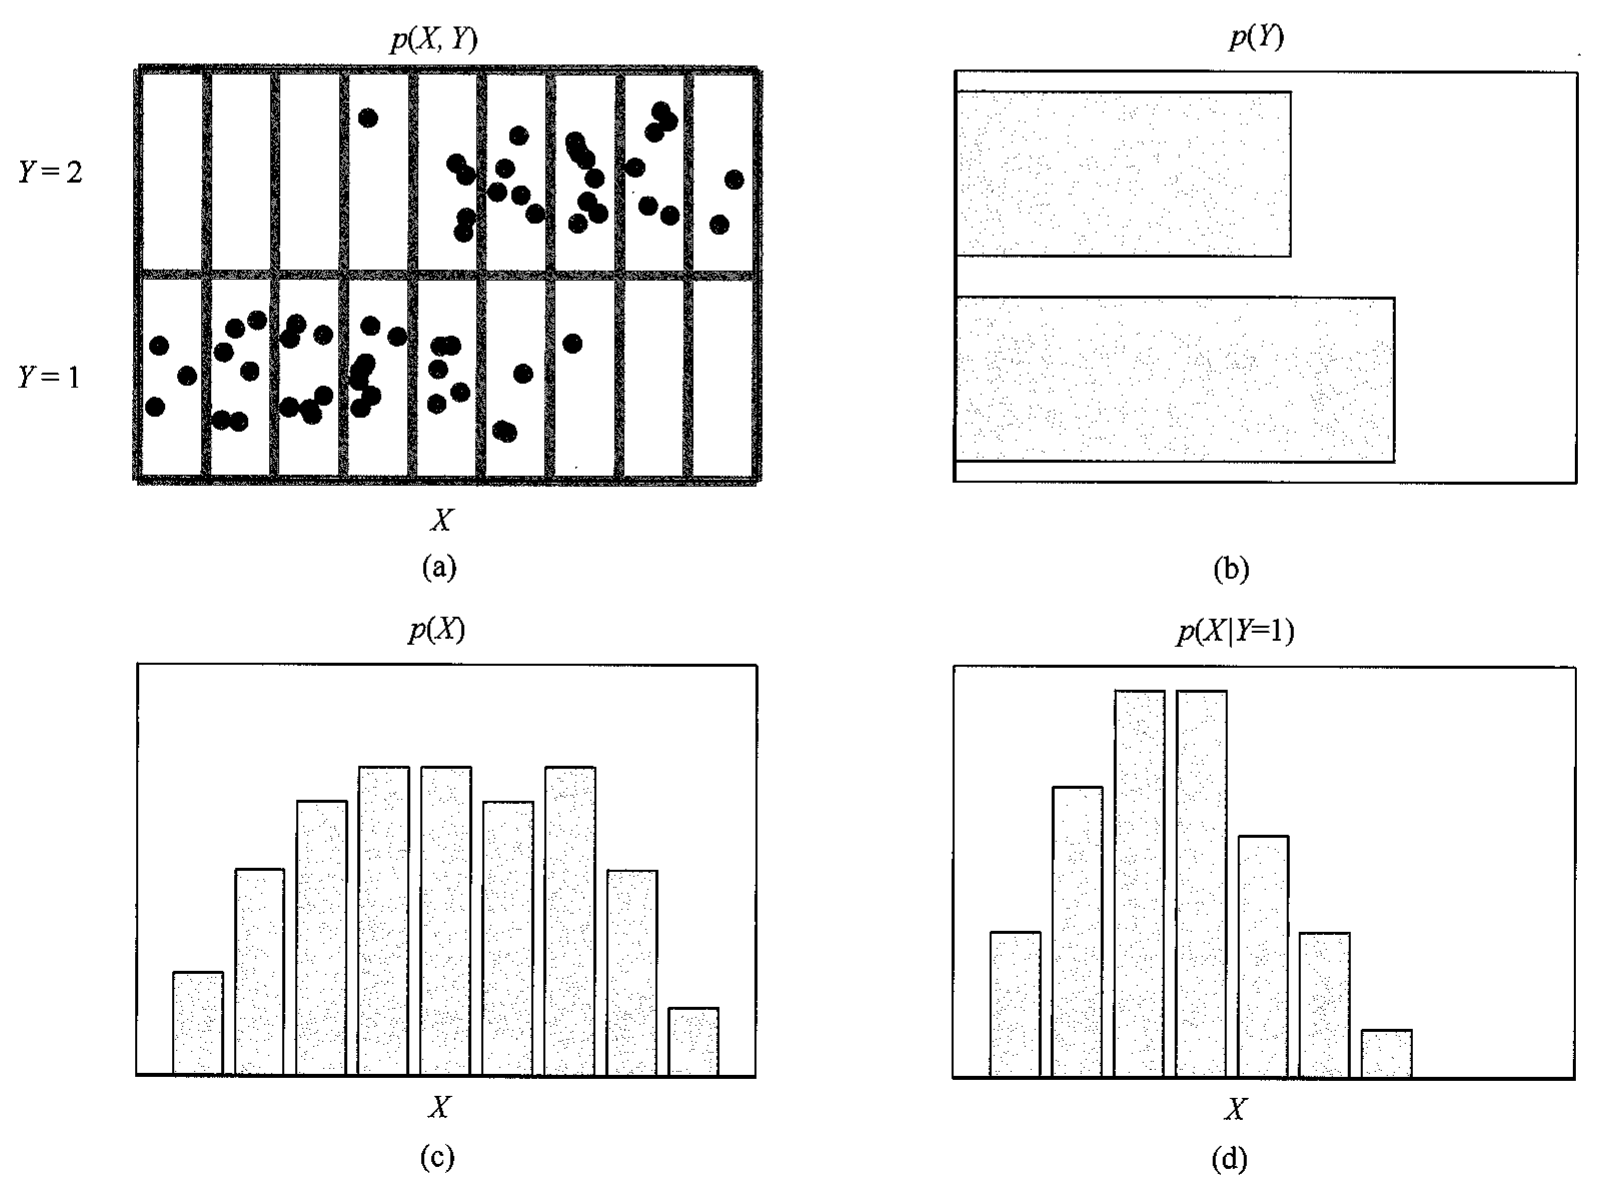
\includegraphics[width=0.95\textwidth]{ch02-fig2-5-joint-marginal.png}
  \caption{变量 $X$ 和 $Y$ 分布的图示。$X$ 有 $9$ 个可能的取值，$Y$ 有 $2$ 个可能的取值。图 (a) 展示了从变量 $X$ 和 $Y$ 的联合分布中抽取的 $60$ 个样本点。图 (b) 和图 (c) 分别展示了边缘分布 $p(Y)$ 和 $p(X)$ 的直方图估计，图 (d) 展示了图 (a) 底部一行所对应的条件分布 $p(X\mid Y=1)$。}
  \label{figure:ch02-联合边缘条件}
\end{figure}

\begin{example}[ 用直方图估计联合、边缘与条件分布]\label{example:ch02-直方图估计}
考虑\cref{figure:ch02-联合边缘条件}中的样本：$X$ 有 $9$ 个可能取值，$Y$ 有 $2$ 个可能取值，从联合分布中抽取 $N=60$ 个点。把样本点按 $X$ 的取值分成 $9$ 列、按 $Y$ 的取值分成 $2$ 行，则：

（1）\cref{figure:ch02-联合边缘条件}(a) 中每个单元格内点的个数除以 $60$，就是该单元格对应取值的联合概率的估计；

（2）把每一行的点数相加再除以 $60$，得到 $p(Y)$ 的估计，即\cref{figure:ch02-联合边缘条件}(b) 中的两个高为 $2/3$ 与 $1/3$ 的长条；

（3）把每一列的点数相加再除以 $60$，得到 $p(X)$ 的估计，即\cref{figure:ch02-联合边缘条件}(c) 中 $9$ 个长条的高度；

（4）只保留 $Y=1$ 那一行（图 (a) 的底部一行），把该行每一列的点数除以该行的总点数，得到条件分布 $p(X\mid Y=1)$ 的估计，即\cref{figure:ch02-联合边缘条件}(d)。

当 $N\to\infty$ 时，这些比例依大数定律收敛到相应的概率，因此直方图是概率分布的一个一致的（但分段常数的）估计。
\end{example}

\begin{remark}（重构新增）
这个例子把\eqref{align:ch02-加和法则}、\eqref{align:ch02-乘积法则}与\eqref{align:ch02-Bayes分母}的差别摆在了同一张图上：图 (b)、(c) 是边缘化（对另一变量求和）的结果，图 (d) 是条件化（只在 $Y=1$ 内重新归一）的结果。二者不可混用——图 (d) 的长条之和为 $1$，而图 (a) 底部一行的点数之和只占全部的 $1/3$。

需要注意，直方图估计的可靠性依赖于箱子的划分：箱子越细，偏差越小但方差越大；这也是\cref{subsection:ch03-直方图}讨论非参数方法时的出发点。
\end{remark}

\subsection{再看医学筛查示例}\label{subsection:ch02-再看医学筛查示例}

让我们回到之前癌症检查的例子，并应用概率的加和法则和乘积法则来回答\cref{subsection:ch02-医学筛查示例}开头提出的两个问题。为了清楚起见，在回答这两个问题时，我们再一次明确区分随机变量和它们的实例。用变量 $C$ 来表示癌症存在与否，它有两个取值：$C=0$ 对应于“未患癌症”，$C=1$ 对应于“患有癌症”。我们假设人群中每 $100$ 人里就有 $1$ 人患有癌症，则有

\begin{align}
  p(C=1) = 1/100 = 0.01
  \label{align:ch02-患癌先验}
\end{align}

\begin{align}
  p(C=0) = 99/100 = 0.99
  \label{align:ch02-未患癌先验}
\end{align}

注意 $p(C=0)+p(C=1)=1$。下面我们引入第二个随机变量 $T$ 来表示检查结果，其中 $T=1$ 为阳性结果，表示检查患有癌症；$T=0$ 为阴性结果，表示检查未患癌症。由\cref{figure:ch02-癌症检查}可知，对于那些患有癌症的人，检查结果呈阳性的概率是 $90\%$；而对于那些未患癌症的人，检查结果呈阳性的概率是 $3\%$。因此，我们可以把这 $4$ 种条件概率都写出来：

\begin{align}
  p(T=1\mid C=1) &= 90/100 = 0.90
  \label{align:ch02-条件概率a}
\end{align}

\begin{align}
  p(T=0\mid C=1) &= 10/100 = 0.10
  \label{align:ch02-条件概率b}
\end{align}

\begin{align}
  p(T=1\mid C=0) &= 3/100 = 0.03
  \label{align:ch02-条件概率c}
\end{align}

\begin{align}
  p(T=1\mid C=1) &= 97/100 = 0.97
  \label{align:ch02-条件概率d}
\end{align}

再次注意，这些概率是归一化的，因此

\begin{align}
  p(T=1\mid C=1) + p(T=0\mid C=1) = 1
  \label{align:ch02-条件归一化C1}
\end{align}

并且同样有

\begin{align}
  p(T=1\mid C=0) + p(T=0\mid C=0) = 1
  \label{align:ch02-条件归一化C0}
\end{align}

\begin{example}[ 癌症检查的定量分析]\label{example:ch02-癌症检查定量}
我们现在可以使用概率的加和法则和乘积法则来回答第一个问题，并估计一个人检查结果呈阳性的概率：

\begin{align}
  p(T=1) &= p(T=1\mid C=0)\,p(C=0) + p(T=1\mid C=1)\,p(C=1) \nonumber \\
  &= \frac{3}{100}\times\frac{99}{100} + \frac{90}{100}\times\frac{1}{100} = \frac{387}{10\,000} = 0.0387
  \label{align:ch02-阳性概率}
\end{align}

可以看到，如果随机找一个人检查，即使他实际患有癌症的概率只有 $1\%$，检查结果呈阳性的概率也大约为 $4\%$。进一步用加和法则可以得到 $p(T=0)=1-387/10\,000=9\,613/10\,000=0.9613$，因此，检查结果呈阴性的概率约为 $96\%$。

再看第二个问题，被检查者往往对此特别关注：如果检查结果呈阳性，那么这个人患有癌症的概率是多少？这需要我们在已有检查结果的条件下估计这个人患有癌症的概率，\eqref{align:ch02-条件概率a}至\eqref{align:ch02-条件概率d}给出了在是否患有癌症的条件下检查结果的概率分布。我们可以使用 Bayes 定理［见\eqref{align:ch02-Bayes定理}］来解决逆向条件概率问题：

\begin{align}
  p(C=1\mid T=1) &= \frac{p(T=1\mid C=1)\,p(C=1)}{p(T=1)}
  \label{align:ch02-后验概率公式}
\end{align}

\begin{align}
  &= \frac{90}{100}\times\frac{1}{100}\times\frac{10\,000}{387} = \frac{90}{387} \approx 0.23
  \label{align:ch02-后验概率数值}
\end{align}

因此，如果一个人的检查结果是阳性，那么他有 $23\%$ 的概率确实患有癌症。应用加和法则，可以得出 $p(C=0\mid T=1)=1-90/387=297/387\approx0.77$，即他有 $77\%$ 的概率实际未患癌症。
\end{example}

\begin{remark}（重构新增）原文问题说明
\eqref{align:ch02-条件概率d}在原书中印作 $p(T=1\mid C=1)=97/100=0.97$，这与\eqref{align:ch02-条件概率a}矛盾（同一个条件概率不可能同时等于 $0.90$ 与 $0.97$），也与\eqref{align:ch02-条件归一化C1}矛盾（$0.90+0.10=1$ 成立，而 $0.97+0.10\neq1$）。结合“$4$ 种条件概率”的上下文与 $97/100$ 这一数值，此处显然应为
\begin{align*}
  p(T=0\mid C=0) = 97/100 = 0.97 ,
\end{align*}
即未患癌症者被正确判为阴性的概率。为保持与原书一致，正文仍按原书字形照录\eqref{align:ch02-条件概率d}；自\eqref{align:ch02-条件归一化C0}起以及本节其余计算（包括\eqref{align:ch02-阳性概率}）均使用修正后的 $p(T=0\mid C=0)=0.97$，两处并不冲突，因为\eqref{align:ch02-条件概率d}的左右两端并未在后续推导中被引用。
\end{remark}

\subsection{先验概率和后验概率}\label{subsection:ch02-先验概率和后验概率}

我们可以用癌症检查的例子对 Bayes 定理做出如下重要解释。如果我们在某人接受检查之前就被问到他是否可能患有癌症，那么我们所能获得的所有信息就是由概率 $p(C)$ 提供的。我们称其为先验概率（prior probability），因为它是在我们观测到检查结果之前可知的概率。一旦这个人的检查结果为阳性，我们就可以使用 Bayes 定理来计算概率 $p(C\mid T)$，我们称其为后验概率（posterior probability），因为它是我们观测到检查结果 $T$ 之后得到的概率。

\begin{definition}[先验概率与后验概率]\label{definition:ch02-先验后验}
在 Bayes 定理\eqref{align:ch02-Bayes定理}中，称 $p(Y)$ 为 $Y$ 的\textbf{先验概率}（prior probability），它是在观测到 $X$ 之前对 $Y$ 的分布的描述；称 $p(Y\mid X)$ 为 $Y$ 的\textbf{后验概率}（posterior probability），它是在观测到 $X$ 之后对 $Y$ 的分布的描述。
\end{definition}

% SUPPLEMENT: parent=definition:ch02-先验后验; kind=motivation; location=紧随其后的 remark（重构新增）
\begin{remark}（重构新增）
“先验”与“后验”是相对于一次观测而言的，不是绝对的：一次推断的后验可以成为下一次推断的先验（这正是 Bayes 方法可以迭代使用的原因，见\cref{section:ch02-Bayes概率}）。在癌症检查中，$p(C=1)=0.01$ 是先验、$p(C=1\mid T=1)\approx0.23$ 是后验，二者相差二十余倍。

后验概率的定义依赖 Bayes 定理，故隐含要求 $p(T=1)>0$：若某种检查结果在总体中不可能出现，就不能据此更新。另外，先验的选择会实质性地影响后验——若人群患癌率不是 $1\%$ 而是 $0.1\%$，同一检查给出的后验会显著降低（见\cref{exercise:ch02-01}）。
\end{remark}

在这个示例中，患有癌症的先验概率是 $1\%$。如果检查结果呈阳性，那么患有癌症的后验概率为 $23\%$。正如我们预期的那样，后者的患癌概率明显更高。尽管从\cref{figure:ch02-癌症检查}来看，检查方法似乎已经非常“准确”了，但检查结果呈阳性的人实际患癌的概率仍然只有 $23\%$（见\cref{exercise:ch02-01}）。这个结论在很多人看来似乎是反直觉的，原因与患有癌症的先验概率较低有关。虽然检查提供了患有癌症的有力证据，但必须通过 Bayes 定理将其与先验概率结合，才能得出正确的后验概率。

\subsection{独立变量}\label{subsection:ch02-独立变量}

如果两个变量的联合分布可以分解为边缘分布的乘积，即 $p(X,Y)=p(X)p(Y)$，则称变量 $X$ 和 $Y$ 是独立的。连续抛掷硬币就是独立事件的一个例子。由乘积法则，有 $p(Y\mid X)=p(Y)$，因此给定 $X$ 下 $Y$ 的条件分布确实独立于 $X$ 的值。在癌症检查样例中，如果检查结果为阳性的概率与此人是否患有癌症无关，则 $p(T\mid C)=p(T)$。这意味着根据 Bayes 定理［见\eqref{align:ch02-Bayes定理}］可得 $p(C\mid T)=p(C)$，因此患癌的概率不会因观测到检查结果而改变。当然，这样的检查是没有用的，因为检查的结果并不能告诉我们这个人是否患有癌症。

\begin{definition}[独立变量]\label{definition:ch02-独立变量}
若两个随机变量 $X$ 和 $Y$ 的联合分布可以分解为它们边缘分布的乘积，即
\begin{align*}
  p(X,Y) = p(X)\,p(Y) ,
\end{align*}
则称 $X$ 和 $Y$ 是\textbf{独立的}。若对任意 $k\geqslant2$，$X_1,\cdots,X_k$ 的联合分布都等于各自边缘分布之积，则称这组变量相互独立。
\end{definition}

% SUPPLEMENT: parent=definition:ch02-独立变量; kind=motivation; location=紧随其后的 remark（重构新增）
\begin{remark}（重构新增）
独立的定义用的是联合分布能否分解，而不是“一个变量不影响另一个变量”这种模糊说法；后者在连续情形下难以直接检验，而分解式是可以计算的。定义对变量的个数没有限制，但两两独立（每个二元组都分解）并不等于相互独立，故需要单独说明 $k$ 元的情形。

定义本身不涉及条件概率，因此不要求 $p(X)>0$；这也说明独立性比“$p(Y\mid X)=p(Y)$”更基本——后者只在 $p(X)>0$ 时才有意义。
\end{remark}

\begin{proposition}[独立性的条件概率刻画]\label{proposition:ch02-独立性刻画}
设 $p(X)>0$。若 $X$ 与 $Y$ 独立，则 $p(Y\mid X)=p(Y)$，即给定 $X$ 后 $Y$ 的条件分布与 $X$ 无关。反之，若对 $X$ 的每个取值都有 $p(Y\mid X)=p(Y)$，则 $X$ 与 $Y$ 独立。
\end{proposition}

\begin{proof}
若 $X$ 与 $Y$ 独立，则由乘积法则\eqref{align:ch02-乘积法则}与独立性的定义，
\begin{align*}
  p(Y\mid X)\,p(X) = p(X,Y) = p(X)\,p(Y) ,
\end{align*}
两边除以 $p(X)>0$ 得 $p(Y\mid X)=p(Y)$。反之，若 $p(Y\mid X)=p(Y)$，代回乘积法则即得 $p(X,Y)=p(X)p(Y)$，故独立。
\end{proof}

% SUPPLEMENT: parent=proposition:ch02-独立性刻画; kind=motivation; location=紧随其后的 remark（重构新增）
\begin{remark}（重构新增）
这条等价刻画解释了“独立”一词的直观含义：知道 $X$ 的取值不会改变 $Y$ 的分布。它也因此给出了独立性的一个实用判据——检查似然比 $p(Y\mid X)/p(Y)$ 是否恒等于 $1$。

在癌症检查中，若检查完全无效（$p(T\mid C)=p(T)$），则由 Bayes 定理得 $p(C\mid T)=p(C)$，观测结果不改变后验，这正是“检查没有提供信息”的精确表述。注意证明用到了 $p(X)>0$；若 $X$ 的某个取值概率为零，该取值上的条件概率本身就没有定义，等价刻画只在正概率取值上成立。
\end{remark}

\end{document}
